\documentclass[thesis.tex]{subfiles}

\begin{document}

\chapter{Spherical ornstein}

Not published, work in progress

\section{Equation of motion}
The unit vector $\ve n$ points in the direction of the symmetry axis of the particle. For sufficiently small particles, the orientational degrees of freedom are driven by the flow gradient $\ma A(\ve r, t) = \nabla \ve u(\ve r, t)$ at the particle position. 
\begin{align*}
	&\ma O = \frac{1}{2}(\ma A - \ma A\transpose),\quad
	\ma S = \frac{1}{2}(\ma A + \ma A\transpose),\quad
	\ma A = \ma O + \ma S
\end{align*}
The equation of motion is then
\begin{align*}
	\dot{\ve n} &= \ma O \ve n + \Lambda (\ma S \ve n - \venn\ma S \ve n)
\end{align*}
In the special case of spherical particles, $\Lambda=0$ and
\begin{align*}
	\dot{\ve n} &= \ma O \ve n. \\
\end{align*}
In dimensionless variables, ($t=\tau t'$, $\ve r = \eta \ve r'$, $\ve u = u_0 \ve u'$, drop primes)
\begin{align*}
	\dot{\ve n} &= \ku\,\ma O \ve n.
\end{align*}
where $\ku = u_0 \tau / \eta$

From implicit solution
\begin{align*}
	\ve n_t &= \ve n_0 + \ku\int_0^t \!\!\rd t_1 \ma O_{t_1} \ve n_{t_1} \\
\end{align*}
expand in $\ku$ by successive replacement of the lhs into rhs.

The autocorrelation function is then
\begin{align*}
	\langle \ve n_0\transpose \ve n_t\rangle &= \ve n_0\transpose\ve n_0 + \ku \int_0^t\!\!\rd t_1 \ve n_0\transpose\langle \ma O_{t_1}\rangle \ve n_0 + \ku^2 \int_0^t\!\!\int_0^{t_1}\!\!\rd t_1\rd t_2 \ve n_0\transpose \langle \ma O_{t_1}\ma O_{t_2}\rangle \ve n_0 + \mathcal O(\ku ^3)
\end{align*}
and so on. To proceed one needs the lagrangian correlation functions of $\ma O$. Simple example
\begin{align*}
	\langle \ma O_{ij}(t) \rangle &= 0,\\
	\langle \ma O_{ij}(0)\ma O_{kl}(t) \rangle &= F_{ijkl}^{OO}\exp(-|t|).
\end{align*}
Then (in three spatial dimensions)
\begin{align}
	\langle \ve n_0\transpose \ve n_t\rangle &= A\left(1 + 5\ku^2 (1-t-e^{-t}) + \mathcal O(\ku ^3)\right)\nn\\
	A &= \ve n_0\transpose\ve n_0,\eqnlab{secular}
\end{align}
For reasons that shortly will be apparent, we leave the initial condition $A=\ve n_0\transpose \ve n_0$ undetermined, even though it is clear that it must be unity for a unit vector.
However, the expansion in \Eqnref{secular} has secular terms, that is terms diverging as $t\to\infty$. 
We know that the correlation function should not diverge, and amend it the following way.

First we factorise the time-independent integration constant $A$ into two time dependent parts
\begin{align}
	A &= \mathcal A (t)\left[1+\ku Z_1(t)+\ku^2 Z_2(t)+\mathcal O(\ku^3)\right] \equiv \mathcal A(t)Z(t)\eqnlab{rg1}
\end{align}
The idea is to insert this into \Eqnref{secular} and use the $Z_i$ to cancel the divergences at each order of \ku, and then use the self-consistency condition that $A$ is time-indpendent, $\dot A=0$, to determine $\mathcal A(t)$ up to the order of perturbation.
Inserting \Eqnref{rg1} into \Eqnref{secular} yields
\begin{align*}
\langle \ve n_0\transpose \ve n_t\rangle &= \mathcal A (t)\left[1+\ku Z_1(t)+\ku^2 Z_2(t)+\mathcal O(\ku^3)\right]\left(1 + 5\ku^2 (1-t-e^{-t}) + \mathcal O(\ku ^3)\right) \\
&= \mathcal A(t)\left[1 + \ku Z_1(t) + \ku^2(Z_2(t)+5(1-t-e^{-t}))+\mathcal O(\ku^3) \right]
\end{align*}
and we choose
\begin{align*}
	Z_1(t) &= 0, \\
	Z_2(t) &= -5(1-t-e^{-t}).
\end{align*}
Then clearly 
\begin{align}
	\langle \ve n_0\transpose \ve n_t\rangle &= \mathcal A (t) + \mathcal O(\ku^3)\eqnlab{rg1a}
\end{align}
but it remains to determine $\mathcal A(t)$ from the self-consistency condition:
\begin{align}
	0 = \dot A &= \dot{\mathcal A}Z + \mathcal A \dot Z \nn\\
	\intertext{which is equivalent to}
	\frac{\rd}{\rd t}\ln\mathcal A &= -\frac{\rd}{\rd t}\ln Z  \nn\\
	\intertext{with solution}
	\mathcal A(t) &= \mathcal A(0) \exp\left(-\ln Z\right)\eqnlab{rg2}
\end{align}
One may of course now conclude, that $\mathcal A=\mathcal A(0)/Z$, but then all we have accomplished is a meaningless algebraic circle from \Eqnref{rg1}. Instead, the correct thing to do is to determine $\ln Z$ up to the order of perturbation, and insert that into \Eqnref{rg2}. In the present case, and in fact for all linear equations, this is rather simple as there exist a mathematical result on logarithms of power series. It says that
\begin{align*}
	\ln \left(1+\ku Z_1(t)+\ku^2 Z_2(t)+\mathcal O(\ku^3)\right) = \ku Y_1(t) + \ku^2 Y_2(t) + \mathcal O(\ku^3)
\end{align*}
and so on, where the new coefficients $Y_n(t)$ are known functions of the $Z_n(t)$, given by the recursive relation\footnote{The $Z_n$ and $Y_n$ are related to the moments and cumulants by $\mu_n = n!Z_n$ and $\kappa_n=n!Y_n$, the recursion relation follows from these identities and standard results on cumulants.}
\begin{align*}
	Y_n = Z_n - \sum_{m=1}^{n-1}\frac{m}{n}Y_mZ_{n-m}
\end{align*}
The first five are included here for reference,
\begin{equation}
\left(
\begin{array}{c}
 Y_1 \\
 Y_2 \\
 Y_3 \\
 Y_4 \\
 Y_5 \\
\end{array}
\right)=
\left(
\begin{array}{c}
 Z_1 \\
 Z_2-\frac{Z_1^2}{2} \\
 \frac{Z_1^3}{3}-Z_2 Z_1+Z_3 \\
 -\frac{1}{4} Z_1^4+Z_2 Z_1^2-Z_3 Z_1-\frac{Z_2^2}{2}+Z_4 \\
 \frac{Z_1^5}{5}-Z_2 Z_1^3+Z_3 Z_1^2+\left(Z_2^2-Z_4\right) Z_1-Z_2 Z_3+Z_5 \\
\end{array}
\right)
\end{equation}
but any number may be easily computed by the Mathematica snippet
\begin{lstlisting}
getYn[n_]:=Z[n]-Sum[m/n getYn[m]Z[n-m],{m,1,n-1}];
Table[getYn[k],{k,1,5}]//Simplify//MatrixForm
\end{lstlisting}
After this slight digression we now know that
\begin{align}
	\ln Z &= \ku Z_1(t) + \ku^2\left(Z_2(t)-\frac{Z_1(t)^2}{2}\right) + \mathcal O(\ku ^3)\nn
	\intertext{in our specific case}
	&= -5\ku^2(1-t-e^{-t})\eqnlab{rg3}
\end{align}
This is now inserted into \Eqnref{rg2}, which in turn determines \Eqnref{rg1a}
\begin{align}
	\langle \ve n_0\transpose \ve n_t\rangle &= \mathcal A (t) + \mathcal O(\ku^3)\nn\\
	&= \mathcal A(0)\exp\left(5\ku^2(1-t-e^{-t})\right)
\end{align}
And finally we can now use the initial condition to determine $\mathcal A(0)=\ve n_0\transpose\ve n_0 = 1$.

\begin{figure}
	\begin{center}
	  \makebox[\textwidth]{%
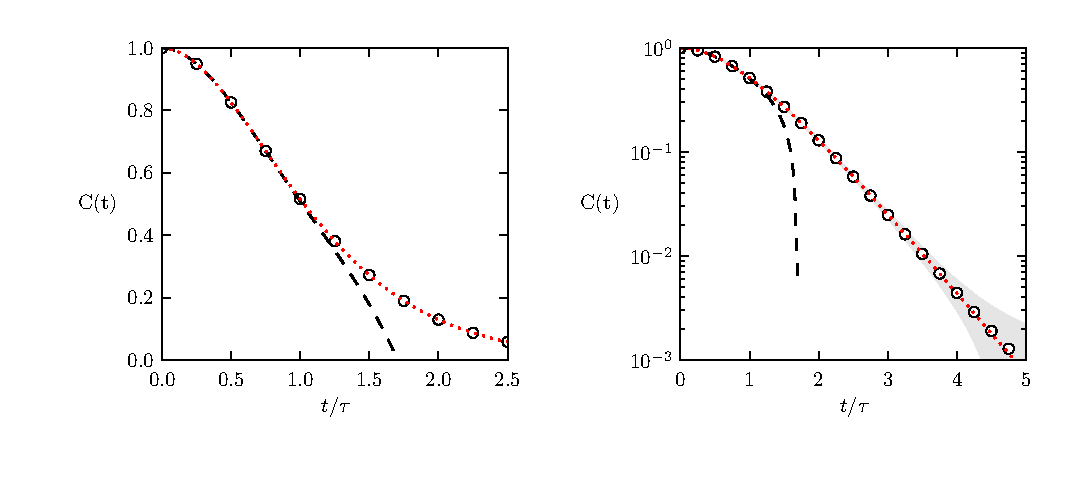
\includegraphics{figs/corr2d_highbeta.pdf}%
}
\end{center}
\caption{\label{fig:corr2d_highbeta} Autocorrelation function of the spherical Ornstein Uhlenbeck process in 2 spatial dimensions. Linear scale (left) and logarithmic scale (right). Numerical simulation open rings, naive perturbation to sixth order dashed line, and fixed perturbation to second order, red dotted line.}%
\end{figure}

\begin{figure}
	\begin{center}
	  \makebox[\textwidth]{%
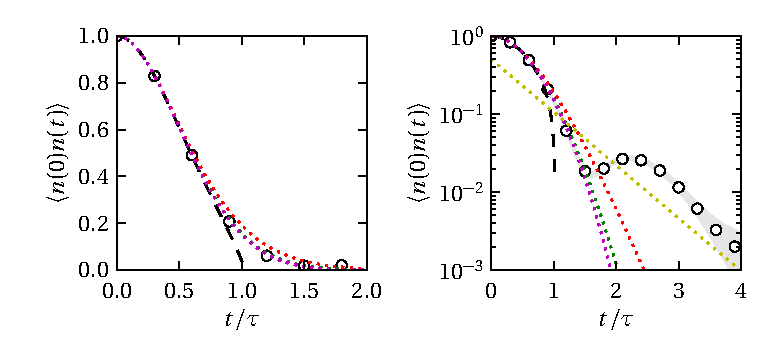
\includegraphics{figs/corr_highbeta.pdf}%
}
\end{center}
\caption{\label{fig:corr2d_highbeta} Autocorrelation function of the spherical Ornstein Uhlenbeck process in 3 spatial dimensions. Linear scale (left) and logarithmic scale (right). Numerical simulation open rings, naive perturbation to sixth order dashed line, and fixed perturbation to second order, red dotted line, fourth order green dotted line, and sixth order magenta dotted line.}%
\end{figure}




\end{document}
